\documentclass[compress]{beamer}
%--------------------------------------------------------------------------
% Common packages
%--------------------------------------------------------------------------
%\usepackage[german]{babel}

% Figures
\usepackage{graphicx}
\graphicspath{{images/}}
\usepackage{subfig}

% Code
\usepackage{listings}
\definecolor{javared}{rgb}{0.6,0,0} % for strings
\definecolor{javagreen}{rgb}{0.25,0.5,0.35} % comments
\definecolor{javapurple}{rgb}{0.5,0,0.35} % keywords
\definecolor{javadocblue}{rgb}{0.25,0.35,0.75} % javadoc
\lstset{
  language=Java,
  showspaces=false,
  showtabs=false,
  breaklines=true,
  showstringspaces=false,
  frame=lines,
  keywordstyle=\color{javapurple}\bfseries,
  commentstyle=\color{javagreen},
  morecomment=[s][\color{javadocblue}]{/**}{*/},
%  keywordstyle=\color{BlueViolet},
%  commentstyle=\color{darkgray},
  identifierstyle=\color{black},
  tabsize = 2,
  stringstyle=\color{javared},
%  stringstyle=\color{Brown},
  escapechar=`,
  columns=fullflexible,
  morekeywords={String, each, and},
  belowskip=0pt,
  basicstyle=\sffamily
}
\definecolor{hlpurple}{RGB}{219,219,204}
\newcommand\hl[1]{\setlength{\fboxsep}{1.5pt}\colorbox{hlpurple}{#1}}

%--------------------------------------------------------------------------
% Load theme
%--------------------------------------------------------------------------
\usetheme{hsrm}

\usepackage{dtklogos} % must be loaded after theme
\usepackage{tikz}
\usetikzlibrary{mindmap,backgrounds}

%\usepackage[english]{babel}

\setbeamercovered{transparent=15}


\title{CodeCatch}
\subtitle{Extracting Source Code Snippets from Online Sources}
\author{Themistoklis Diamantopoulos\\ Georgios Karagiannopoulos\\ Andreas Symeonidis\\ {\small asymeon@eng.auth.gr
}}

\institute{Electrical \& Computer Engineering Dept.\\ Aristotle University of Thessaloniki}

%\date{\today}

\begin{document}

\maketitle

\section*{Contents}
\begin{frame}
	\frametitle{CONTENTS}
	\tableofcontents[hideallsubsections]
\end{frame}

\section{Introduction}

\begin{frame}{Recommendation Systems}
\onslide<1->
The routine process of writing new code involves using search engines to find {\Medium snippets} from websites like StackOverflow, blogs, documentation etc.

\vfill
This approach is time-consuming, distracting, and implies a lot of personal effort by the developer.

\onslide<2->
\vfill
{\Medium CodeCatch}: A system that accelerates the process of searching and separating the solutions for a specific programming task.


\end{frame}

\begin{frame}{Related Work}
\onslide<1->
Many similar systems have been proposed in the past:

\quoted {Prospector, PARSEWeb, MAPO, UP-Miner, PAM, APIMiner, eXoaDocs, DECKARD, Blueprint, ...}

\alert{Deficits} of the aforementioned systems:

\onslide<2->
\begin{itemize}
	\item Too much knowledge is required beforehand for the API to be used.
	\item Most of them do not return ready-to-use snippets.
	\item Results are presented in form of lists, setting the different implementations difficult to separate.
	\item They preserve local indexes with limited size and diversity and sometimes outdated.
	\item Quality and reusability of results usally not evaluated.
	\item They involve some specialized query language requiring additional effort.
\end{itemize}

\end{frame}

\section{CodeCatch}
\begin{frame}{CodeCatch System Overview}

\begin{figure}
	\centering
	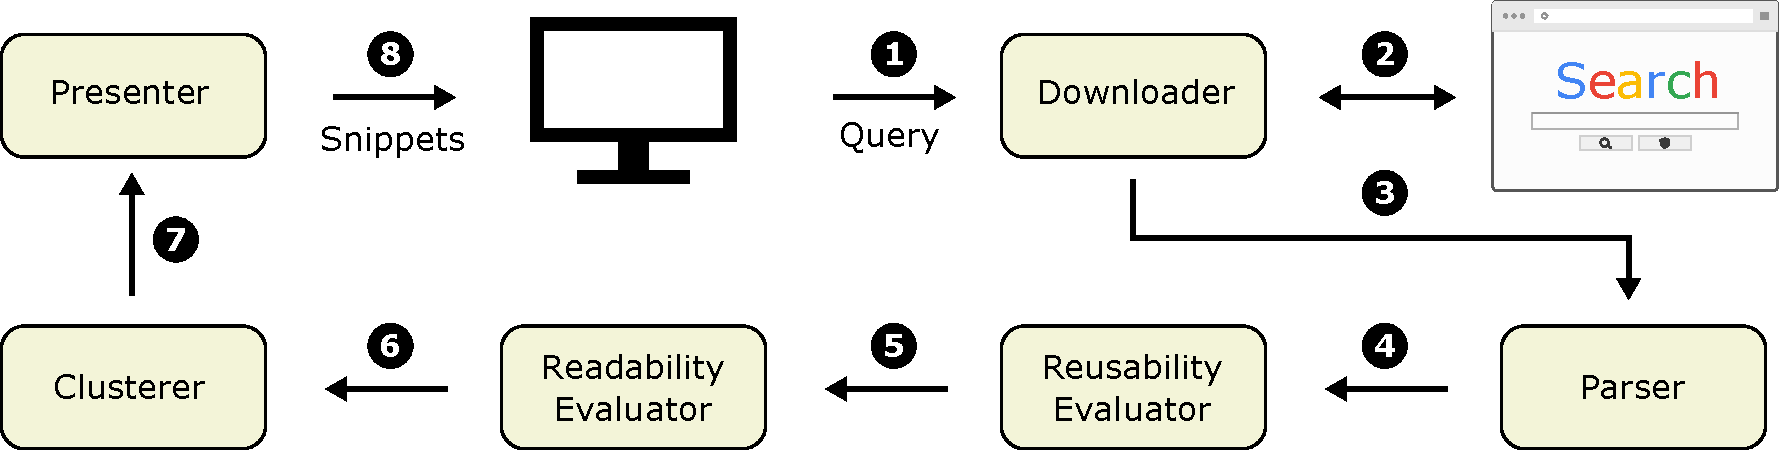
\includegraphics[width=\textwidth]{systemoverviewnew}
	\caption{The components of CodeCatch and how they are connected.}
\end{figure}

\end{frame}

%%%%%%%%%%%%%%%%%%%%%%%%%%%%%%%%%%%%%%%%%%%%%%

\begin{frame}{Downloader}


\begin{figure}[t]
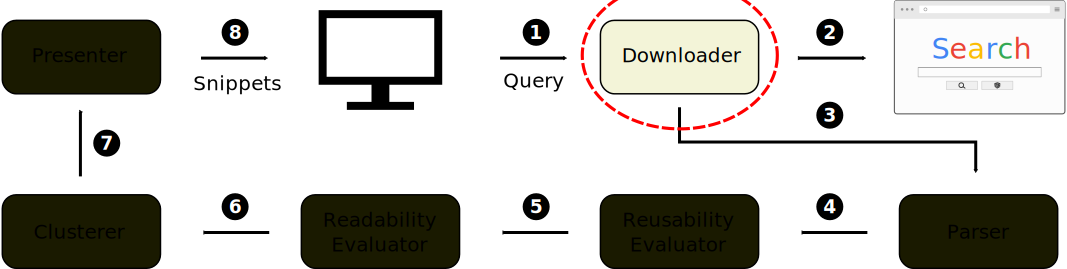
\includegraphics[scale=0.33]{downloader}
\end{figure}

\begin{block}{Functionality of Downloader}
\begin{enumerate}
	\item Receives as input the query of the developer in natural language (e.g. \textit{"How to read a CSV file"}).
	\item Augments the query with Java-related keywords in order to retrieve more relevant results.
	\item Issues the query in the search engine and scrapes the returned web pages.
\end{enumerate}
\end{block}


\end{frame}
%%%%%%%%%%%%%%%%%%%%%%%%%%%%%%%%%%%%%%%%%%%%%%

\begin{frame}{Parser}
	\vspace{-8pt}
	\begin{figure}[t]
	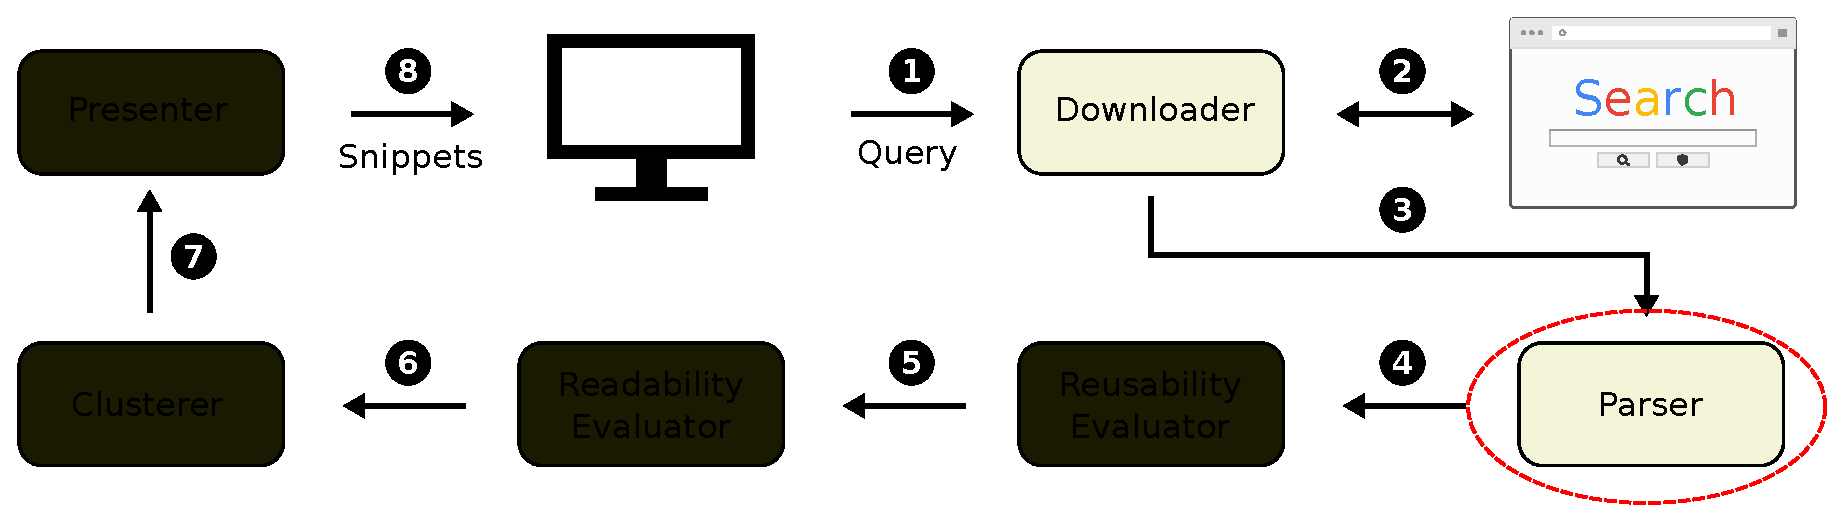
\includegraphics[scale=0.3]{parser}
	\end{figure}
	
	\vspace{-8pt}
	\begin{block}{Functionality of Parser}
	\begin{enumerate}
		\item Extracts the Abstract Syntax Tree (AST) of each snippet.
		\item One pass over AST to extract type declarations and one pass to extract API calls.
		\item Drops any snippets not referring to Java source code or not producing API calls.
	\end{enumerate}
	\end{block}
		
	{\Medium Note}: The parser is robust even when the snippets are not compilable.
\end{frame}

%%%%%%%%%%%%%%%%%%%%%%%%%%%%%%%%%%%%%%%%%%%%

\begin{frame}{Reusability Evaluator}

   	\begin{figure}[t]
	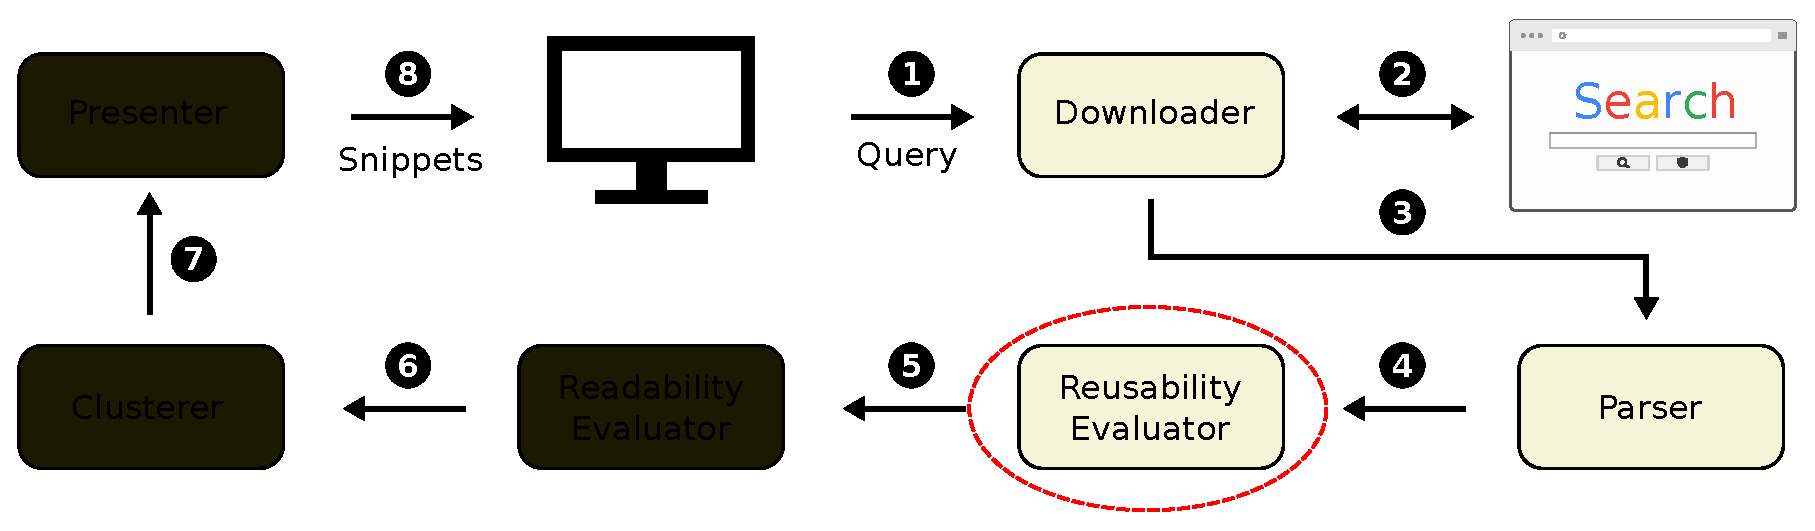
\includegraphics[scale=0.35]{reusability}
    \end{figure}

 	\only<1>{
		\begin{exampleblock}{Notion behind evaluating reusability...}
			{\Medium Assumption}: Snippets with API calls commonly used by other developers are more probable to be of reuse.\\
			{\Medium Reason}: Frequently used APIs usually indicate common practice, thus are prone to be reused in different projects.
		\end{exampleblock}
    }

	\only<2>{
		\vspace{-10pt}	
		\begin{block}{Functionality of Reusability Evaluator}
			\begin{enumerate}
				\item We download locally a set of high-quality projects.
				\item We construct a local index where we store their API calls, extracted using the Parser.
				\item We calculate the appearence frequency of each API call.
				\item We evaluate the reusability of each snippet by averaging the scores of its API calls.
			\end{enumerate}
		\end{block}
	}
\end{frame}

%%%%%%%%%%%%%%%%%%%%%%%%%%%%%%%%%%%%%%%%%
\begin{frame}{Readability Evaluator}

   	\begin{figure}[t]
	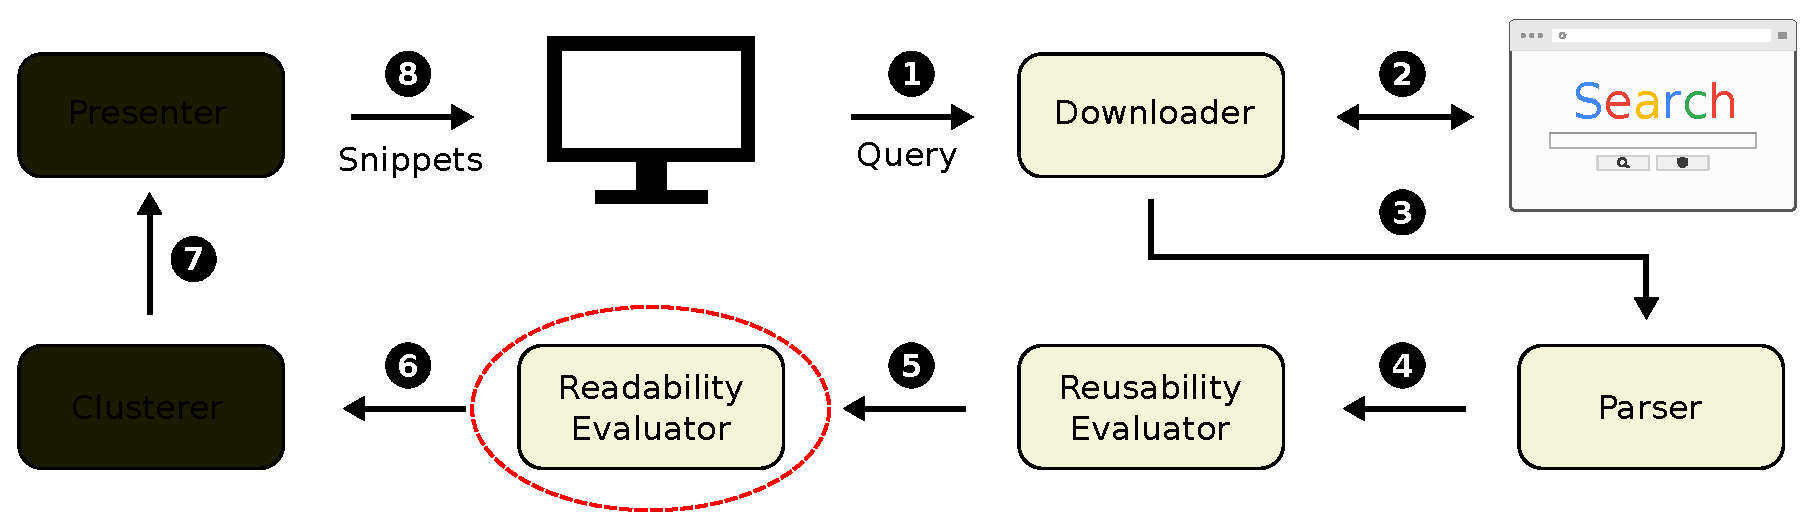
\includegraphics[scale=0.35]{readability}
    \end{figure}
	
	\only<1>{
	\begin{exampleblock}{Definition}
	We define {\Medium readability} as the human judgement of how easy a text is to understand.
	\end{exampleblock}

	\doublequoted{Our target is to build a {\Medium classifier} using supervised-learning and a dataset of 	annotated snippets regarding their readability, which will be capable of judging the readability of new unseen snippets.}
	}
	
	\only<2>{
	\vspace{-10pt}
	\begin{block}{Functionality of Readability Evaluator}
		\begin{enumerate}
			\item We extract a set of 25 features that are related to readability (e.g. avg identifier length, avg number of comments, etc.
			\item We build a binary classifier using AdaBoost and decision trees. The training was done on a publicly available dataset.
			\item We evaluate the readability of new snippets using our trained model with 85\% F-Measure score.
		\end{enumerate}

	\end{block}
	}
	
\end{frame}
%%%%%%%%%%%%%%%%%%%%%%%%%%%%%%%%%%%%%%%%%

\begin{frame}{Clusterer}

\begin{figure}[t]
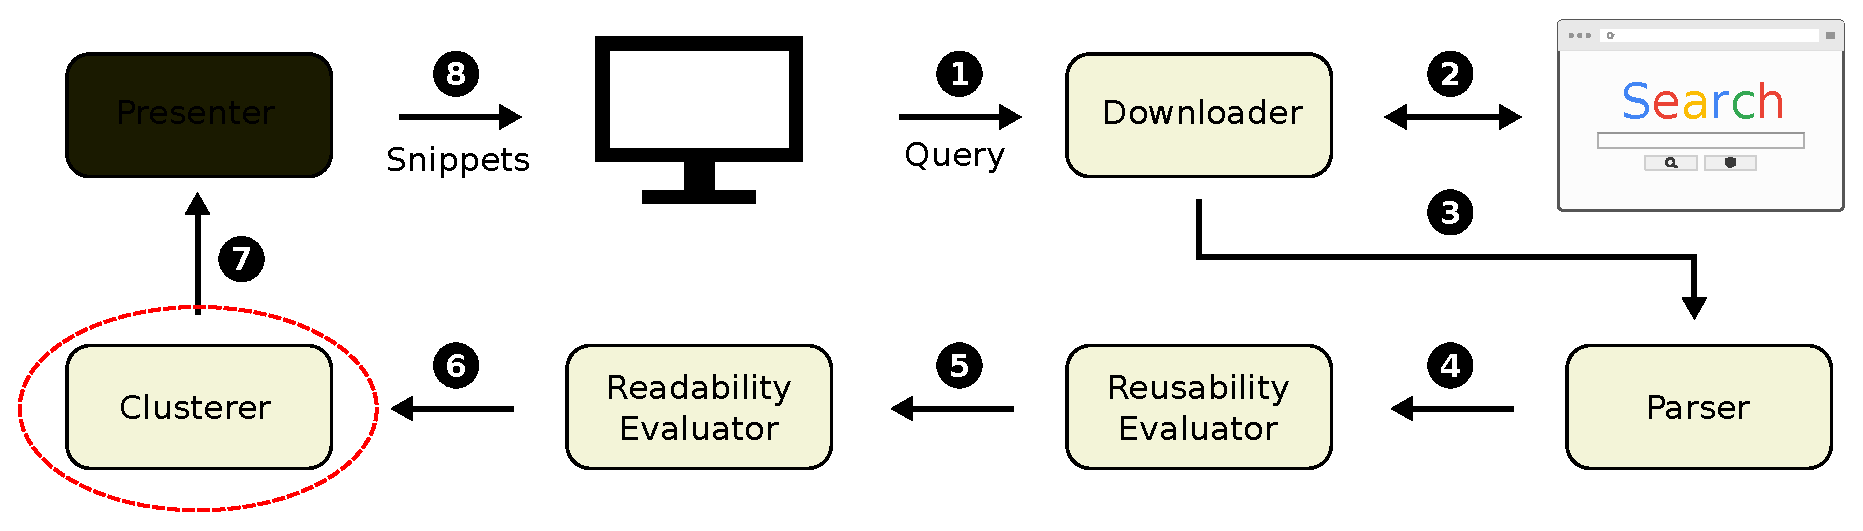
\includegraphics[scale=0.35]{clusterer}
\end{figure}

\doublequoted{Our target is to cluster the retrieved snippets based on their different implementations to the problem.}

\onslide<2->
\begin{exampleblock}{Assumption...}
...snippets which use different API calls represent different implementations of the problem.
\end{exampleblock}

\end{frame}

%%%%%%%%%%%%%%%%%%%%%%%%%%%%%%%%%%%%%%%%%

\begin{frame}[fragile]
\frametitle{Clustering}

\begin{lstlisting}[language=Java,basicstyle=\tiny]
String line = "";
BufferedReader br = null;
try {
    br = new `\hl{BufferedReader}`(new `\hl{FileReader}`("test.csv"));
    while((line = br.`\hl{readLine}`()) != null) {
        String[] data = line.split(",");
    }
    br.`\hl{close}`();
} catch (Exception e) {
    System.err.println("CSV file cannot be read: " + e);
}
\end{lstlisting}

\begin{lstlisting}[language=Java,basicstyle=\tiny]
Scanner scanner = null;
try{
    scanner = new `\hl{Scanner}`(new `\hl{File}`("test.csv"));
    scanner.useDelimiter(",");
    while(scanner.`\hl{hasNext}`()) {
        System.out.print(scanner.`\hl{next}`() + " ");
    }
    scanner.`\hl{close}`();
} catch (Exception e) {
    System.err.println("CSV file cannot be read: " + e);
}
\end{lstlisting}

Clustering snippets by examining them as plain text documents is \alert{not efficient}! About 60\% common tokens in both snippets...

\end{frame}

%%%%%%%%%%%%%%%%%%%%%%%%%%%%%%%%%%%%%%%%%%%%%%%%%%%%%%%%%

\begin{frame}{Clusterer}

\begin{block}{Preprocessing \& Clustering}
\begin{enumerate}
	\item We represent each snippet as a vector in a {\Medium Vector Space Model} (VSM) with respect to its API calls.
	\item We use a {\Medium tf-idf} vectorizer to extract the vector representation for each document.
	\item We calculate the distance between snippets measuring the {\Medium cosine similarity}.
	\item We perform {\Medium silhouette analysis} in order to determine the optimal number of clusters.
	\item We employ {\Medium K-Means} algorithm for the final clustering, as it is known to be effective in text clustering problems like ours.
	
\end{enumerate}
\end{block}

\end{frame}

%%%%%%%%%%%%%%%%%%%%%%%%%%%%%%%%%%%%%%%%%%%%%%%%%%%%%%%%%
\begin{frame}{Example silhouette analysis}

\begin{figure}
\def\thewidth{0.5\textwidth}
 \centering
 \subfloat[][]{
 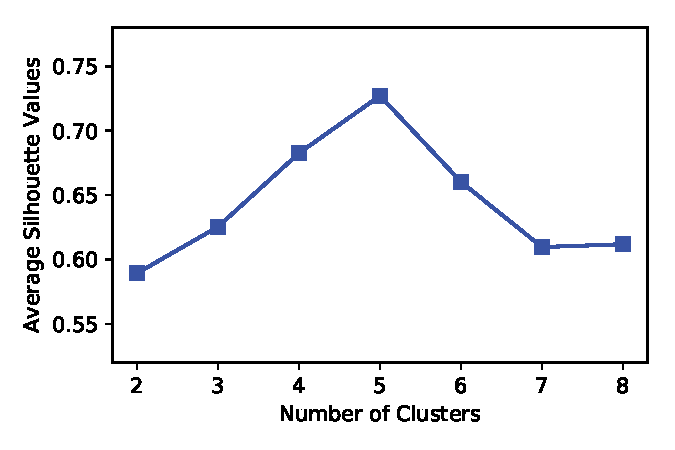
\includegraphics[width=\thewidth]{images/silhouetteFull}
 \label{fig:silhouetteFull}
 }
 \subfloat[][]{
 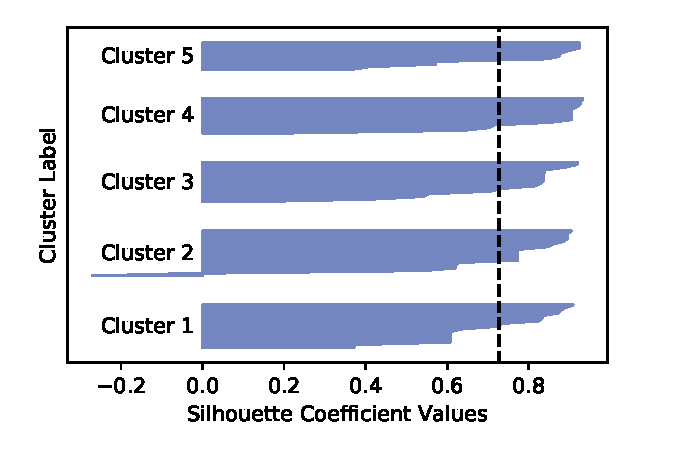
\includegraphics[width=\thewidth]{images/silhouette}
 \label{fig:silhouette}
 }
 \caption[]{Example silhouette analysis for clustering the snippets of query "How to read a CSV file", including~\subref{fig:silhouetteFull} the silhouette score for different number of clusters and~\subref{fig:silhouette} the silhouette of each of the 5 clusters.}
 \label{fig:silhouetteAnalysis}
\end{figure}

\end{frame}

%%%%%%%%%%%%%%%%%%%%%%%%%%%%%%%%%%%%%%%%%%%%%%%%%%%%%%%%%

\begin{frame}{Presenter}

\vspace{-20pt}
\begin{figure}[t]
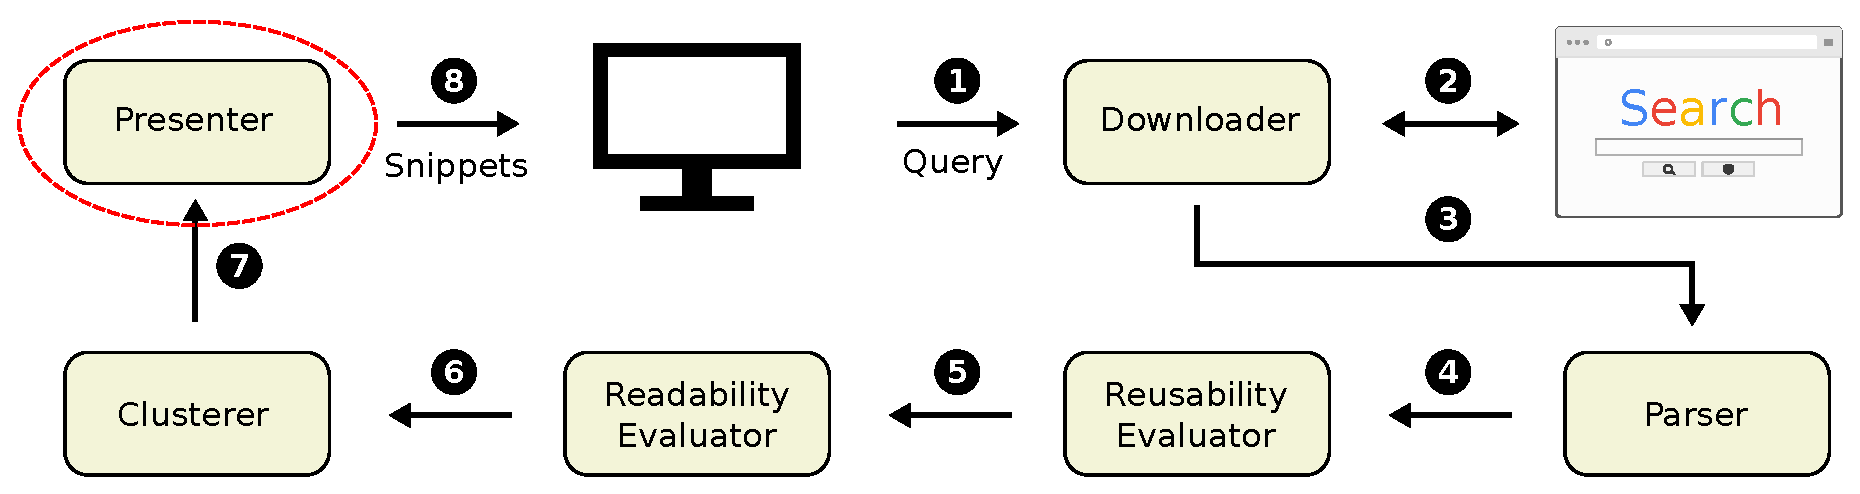
\includegraphics[scale=0.35]{presenter}
\end{figure}

\doublequoted{The presenter handles the ranking and the presentation of the results.}

\begin{exampleblock}{Ranking}
The snippets within a cluster are ranked according to their API reusability score, and in cases of equal scores according to their distance from the cluster centroid.\\
The overall cluster score emerges from averaging the scores of its containing snippets. 
\end{exampleblock}

\end{frame}

%%%%%%%%%%%%%%%%%%%%%%%%%%%%%%%%%%%%%%%%%%%%%%%%%%%%%%%%%
\begin{frame}{Presenter}

\doublequoted{User inserts in CodeCatch the query {\Medium "How to read CSV file"} and initially gets presented with the clusters formed.}

\only<1>{
\begin{figure}
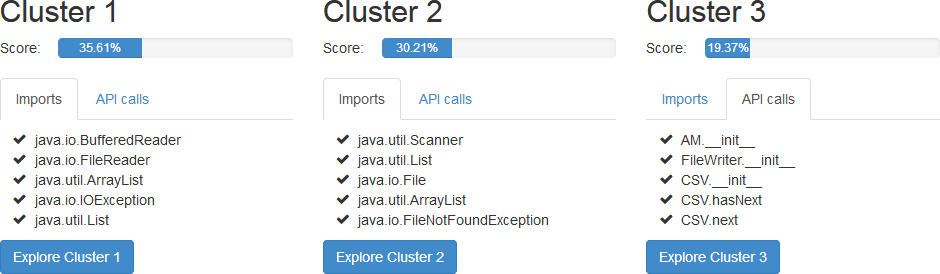
\includegraphics[width=\textwidth]{screenshotclusters}
\end{figure}
}

\only<2>{
\begin{figure}
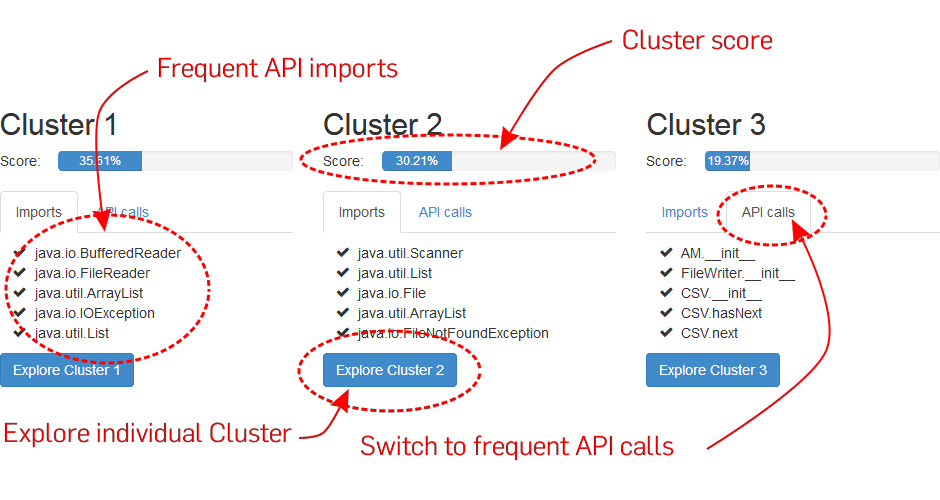
\includegraphics[width=\textwidth]{screenshotclusters4}
\end{figure}
}

\only<3>{
\begin{figure}
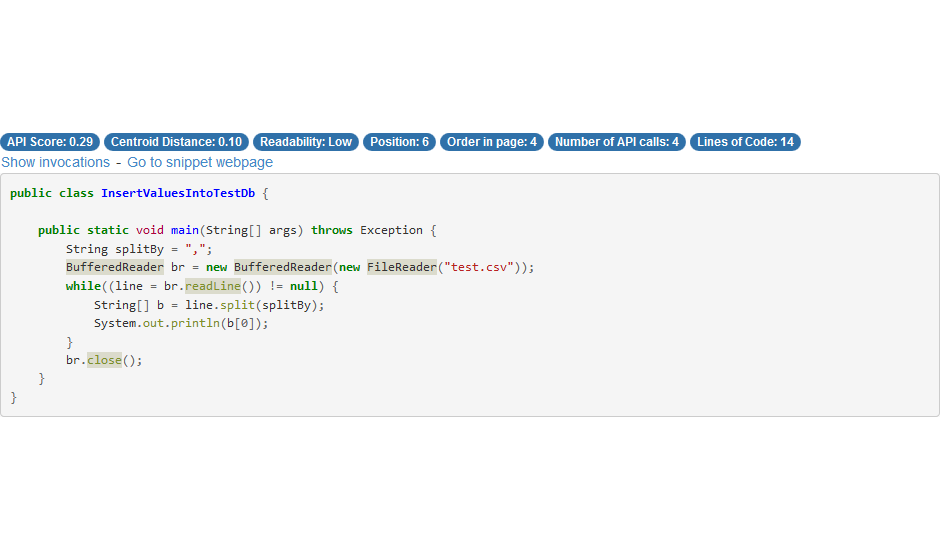
\includegraphics[width=\textwidth]{screenshotsnippet1}
\end{figure}
}

\only<4>{
\begin{figure}
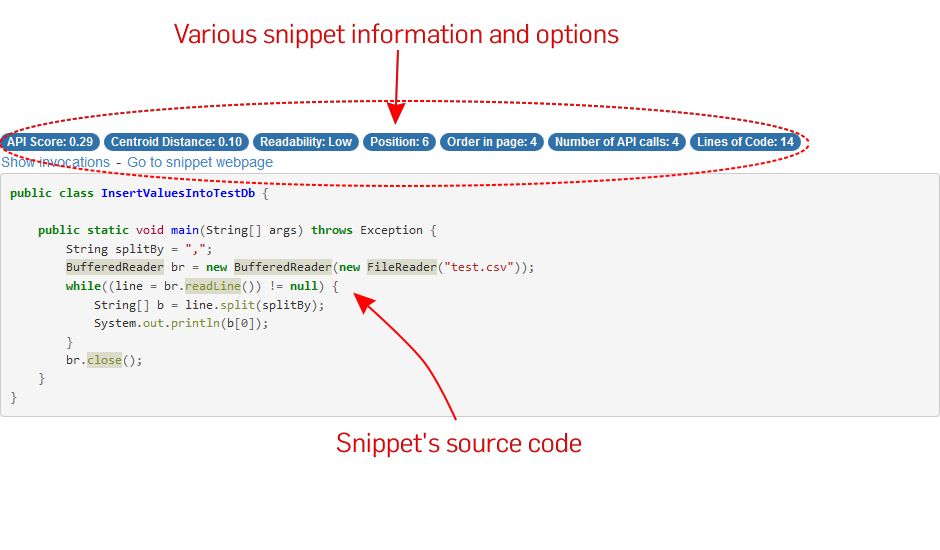
\includegraphics[width=\textwidth]{screenshotsnippet2}
\end{figure}
}

\end{frame}
%%%%%%%%%%%%%%%%%%%%%%%%%%%%%%%%%%%%%%%%%%%%%%%%%%%%%%%%%

\section{System Evaluation}

%%%%%%%%%%%%%%%%%%%%%%%%%%%%%%%%%%%%%%%%%%%%%%%%%%%%%%%%%
\begin{frame}{Evaluation Framework}

\onslide<1->
The purpose of our evaluation is:
\begin{itemize}

	\item To assess whether the snippets of our snippets are relevant.
	\item To determine whether the developer can indeed more easily find snippets for all different APIs relevant to a query.
	
\end{itemize}


\onslide<2->
We perform reusability-related evaluation against Google search engine on a dataset of common queries.

\begin{table}
\centering
\tiny
\begin{tabular}{ c l c c c c }
\hline
\textbf{Index} & \textbf{Query} & \textbf{Clusters} & \textbf{Snippets} & \textbf{Snippets/Cluster}\\
\hline
1 & How to read CSV file & 3 & 44 & 14.7\\
2 & How to generate MD5 hash code & 4 & 43 & 10.8\\
3 & How to upload file to FTP & 3 & 13 & 4.3\\
4 & How to split string & 5 & 53 & 10.6\\
5 & How to draw text graphics & 3 & 40 & 13.3\\
6 & How to play audio file & 5 & 79 & 15.8\\
7 & How to substitute string & 3 & 31 & 10.3\\
8 & How to convert collection to an array & 4 & 49 & 12.3\\
9 & How to send email & 3 & 46 & 15.3\\
10& How to connect to a JDBC database & 5 & 44 & 8.8\\
11& How to execute select statement JDBC database & 3 & 59 & 19.7\\
12& How to initialize thread & 3 & 33 & 11.0\\
13& How to write binary data & 3 & 35 & 11.7\\
14& How to read ZIP archive & 2 & 32 & 16.0\\
15& How to send packet via UDP & 2 & 31 & 15.5\\
\hline
\end{tabular}
\end{table}

\end{frame}

%%%%%%%%%%%%%%%%%%%%%%%%%%%%%%%%%%%%%%%%%%%%%%%%%%%%%%%%%

\begin{frame}{Evaluation Framework}

\begin{itemize}

\item The annotation procedure was performed without any knowledge on the ranking of snippets in order to maintain an objective outlook.

\pause

\item Snippets were marked as {\Medium relevant} iff their code covers the functionality described by the query.

\pause
\item  We consider that the user examines the results subsequently (i.e. as a list of results) for both systems.

\pause
\item For further the assessment of each cluster, we annotate the results to consider them relevant for each implementation.

\pause
\item We use {\Medium reciprocal rank} as a metric for comparison.

\end{itemize}

\end{frame}

%%%%%%%%%%%%%%%%%%%%%%%%%%%%%%%%%%%%%%%%%%%%%%%%%%%%%%%%%

\begin{frame}{Evaluation Results}

\begin{figure}
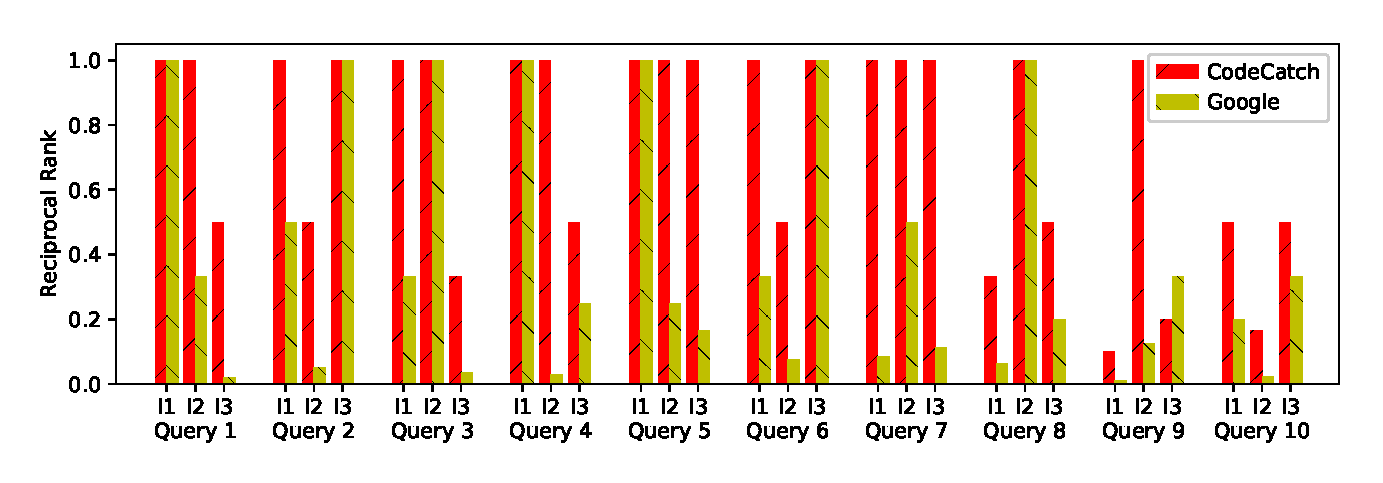
\includegraphics[width=\textwidth]{reciprocalrank}
\caption[]{Reciprocal Rank of CodeCatch and Google for the three most popular implementations (I1, I2, I3) of each query.}
\end{figure}

\doublequoted{Reciprocal Rank (RR) is computed as the inverse of the rank of the first relevant result ($RR = \frac{1}{rank}$).}


\end{frame}

%%%%%%%%%%%%%%%%%%%%%%%%%%%%%%%%%%%%%%%%%%%%%%%%%%%%%%%%%


\begin{frame}{Evaluation Conclusions}

\begin{figure}
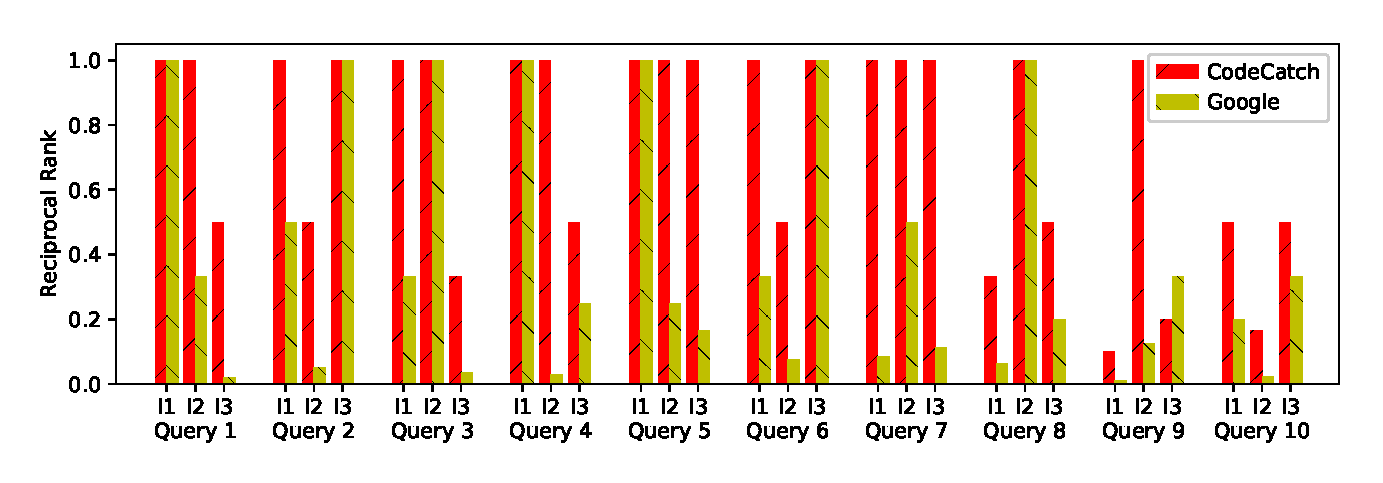
\includegraphics[scale=0.45]{reciprocalrank}
\end{figure}

\vspace{-5pt}
\begin{itemize}
	\item In terms of the {\Medium relevance} of the results both systems are very effective.
	\pause
	\item In some cases (e.g. Q1 - "How to read CSV file") developers can find relevant snippets for different implementations using CodeCatch {\Medium quicker}.
	\pause
	\item CodeCatch places the {\Medium most popular} implementation at the top of the list more often than Google (e.g. queries 2, 3, 6, 7, 10).

\end{itemize}

\end{frame}
%%%%%%%%%%%%%%%%%%%%%%%%%%%%%%%%%%%%%%%%%%%%%%%%%%%%%%%%%

\begin{frame}{Conclusions - Future Work}

Conclusion from our work:

\begin{itemize}
	\item Software engineers can save valuable time using recommendation systems.
	\item Assessing the readability and reusability can improves the quality of results.
	\item Grouping results into clusters provides a comprehensive view of the different implementations. 
\end{itemize}

\pause

Future work could be directed into:

\begin{itemize}
	\item Improving the ranking scheme to include further information (e.g. developer's preference)
	\item Performing snippet summarization using information from the clustering.
	\item Conducting a developer study in order to further assess CodeCatch for its effectiveness.
\end{itemize}

\end{frame}

\begin{frame}

\begin{center}
CodeCatch web application is available at:\\
{\Medium http://codecatch.ee.auth.gr}\\
\vfill
We thank you for your attention!\\
Questions?\\


\end{center}
\end{frame}

\end{document}






